\documentclass[a4paper, 12pt, oneside]{book}

\usepackage[italian]{babel}
\usepackage[T1]{fontenc}
\usepackage[utf8]{inputenc}
\usepackage{graphicx}

\usepackage{color}
\usepackage{listings}

\author{Marco Ferraioli \and Dario Tecchia}
\title{Design Pattern}
\date{2015-16}

\definecolor{mygreen}{rgb}{0,0.6,0}
\definecolor{mygray}{rgb}{0.5,0.5,0.5}
\definecolor{mymauve}{rgb}{0.58,0,0.82}
\definecolor{whitesmoke}{RGB}{236,236,236}

\lstset{ %
  numbers=left,
  backgroundcolor=\color{whitesmoke},   % choose the background color
  basicstyle=\footnotesize,             % size of fonts used for the code
  breaklines=true,                      % automatic line breaking only at whitespace
  captionpos=b,                         % sets the caption-position to bottom
  commentstyle=\color{mygreen},         % comment style
  escapeinside={\%*}{*)},               % if you want to add LaTeX within your code
  keywordstyle=\color{blue},            % keyword style
  stringstyle=\color{mymauve},          % string literal style
}

\begin{document}

  \begin{titlepage}
    \centering
    
\includegraphics[width=0.20\textwidth]{img/python-logo.png}\par\vspace{1cm}
    {\scshape\LARGE Università degli Studi di Salerno \par}
    \vspace{1cm}
    {\scshape\Large Tesina Design Pattern\par}
    \vspace{1.5cm}
    {\huge\bfseries Adapter Pattern\par}
    \vspace{2cm}
    {\Large\itshape M.~Ferraioli D.~Tecchia\par}
    \vfill

    \vfill

  % Bottom of the page
    {\large 2015-16\par}
  \end{titlepage}

  %\maketitle
  \tableofcontents
  
  \chapter{Pattern Strutturali}

I pattern strutturali consentono di riutilizzare degli oggetti 
esistenti fornendo agli utilizzatori un'interfaccia più adatta alle 
loro esigenze.

I design patterns strutturali possono essere basati su classi o oggetti:
Quelli basati su classi utilizzano l’ereditarietà per generare classi 
che combinano le proprietà di classi base, mentre, quelli basati su oggetti 
mostrano come comporre oggetti per realizzare nuove funzionalità.

  \section{Adapter Pattern}
  
    \subsection{Introduzione e Scopo}
    
    L'Adapter Pattern, conosciuto anche come Wrapper, ha il fine di fornire
    una soluzione astratta al problema dell'interoperabilità tra interfacce 
    differenti.
    
    Il problema si presenta ogni qual volta nello sviluppo di un software 
    si devono utilizzare sistemi di supporto (come per esempio librerie)
    di terze parti la cui interfaccia non è perfettamente compatibile con 
    quella richiesta da software già esistenti senza poter andare a 
    riscrivere parte del sistema. Anche se quest'ultima possibilità fosse
    possibile sarebbe comunque un compito oneroso.
    
    \subsection{Partecipanti}
    
    L'Adapter pattern ha in totale quattro partecipanti:
    \begin{description}
      \item[Adaptee] \hfill \\
      Indica un’esistente interfaccia che ha bisogno di essere adattata; 
      esso rappresenta il componente con il quale il client vuole interagire.
      
      \item[Target] \hfill \\
      Indica l’interfaccia specifica del dominio che utilizza il client; 
      fondamentalmente rappresenta l’interfaccia dell’Adapter che aiuta il 
      client ad interagire con l’Adaptee.

      \item[Adapter] \hfill \\
      Adatta l’interfaccia Adaptee all’interfaccia Target; 
      in altre parole, implementa l’interfaccia di Target, e connette 
      Adaptee con il client.

      \item[Client] \hfill \\
      Il client principale che vuole ottenere l’operazione.
      
    \end{description}
    
    \subsection{Class Adapter e Object Adapter} \hfill
    
    Possiamo avere due tipi di Adapter Pattern:
    \begin{itemize}
      \item Class Adapter
      \item Object Adapter
    \end{itemize}
    
    La principale differenza sta nel fatto che il Class Adapter usa il 
    concetto dell’ereditarietà, mentre l’Object Adapter usa il concetto 
    della composizione.
  
    \paragraph{Class Adapter} \hfill \\
    Il \emph{Class Adapter}, come accennato, utilizza l’ereditarietà 
    multipla e può contenere una sola classe. 
    Non può contenere un’interfaccia poiché per 
    definizione deve derivare da qualche classe base:
    
    \begin{figure}[htbp]
      \begin{center}
        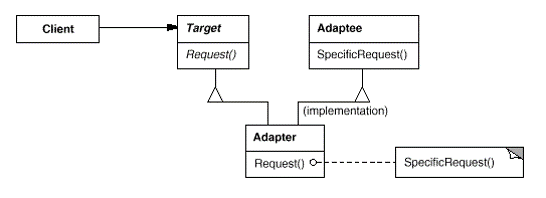
\includegraphics[width=12cm]{img/umls/class_adapter.png}
      \end{center}
      \caption{UML Class Adapter}
      \label{fig:dessin}
    \end{figure}
    
    \paragraph{Object Adapter} \hfill \\
    L’\emph{Object Adapter} si basa sulla composizione di oggetti e può 
    contenere interfacce o classi, o entrambe.
    
    \begin{figure}[htbp]
      \begin{center}
        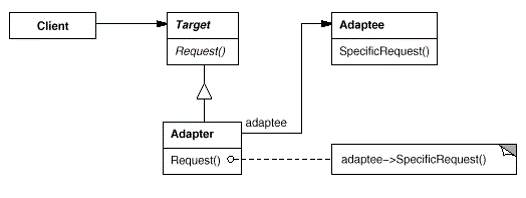
\includegraphics[width=12cm]{img/umls/object_adapter.png}
      \end{center}
      \caption{UML Object Adapter}
      \label{fig:dessin}
    \end{figure}
    
    \subsection{Quando è importante usare il Pattern}
    Possiamo concludere sicuramente, che l'Adapter Pattern risulta un'ottima
    scelta quando:
    
    \begin{itemize}
      
      \item Vogliamo usare classi esistenti, e le loro
      interfacce non sono compatibili con quelle di cui abbiamo bisogno.
      Per esempio quando si deve usare del codice di terze parti non 
      pienamente compatibile con il codice del client.
    
      \item Si vogliono creare classi riutilizzabili che cooperino con 
      classi impreviste e che non hanno necessariamente interfacce 
      compatibili.
      
      \item Si vogliono usare parecchie sottoclassi esistenti, ma risulta 
      poco pratico adattare la loro interfaccia facendo sottoclassi di ognuna. 
      Un Object Adapter può adattare l’interfaccia della sua superclasse. 
      Valido solo per Object Adapter.
      
      \item Un Object Adapter può essere utilizzato per un codice 
      che usa classi legacy. Invece, Il Class Adapter viene utilizzato se si ha bisogno 
      dell’ereditarietà singola.
    
    \end{itemize}
    
    \subsection{Vantaggi del Pattern}
    
    Per quanto riguarda i vantaggi di questo pattern, nel caso del 
    \emph{Class Adapter} abbiamo l'istanziazione di un solo nuovo oggetto,
    meno codice rispetto all'Object Adapter, e la 
    possibilità di fare l'override dei metodi di \emph{Adaptee}; invece,
    per l'\emph{Object Adapter} possiamo dire che è più flessibile rispetto
    al \emph{Class Adapter} e non richiede l'impiego di sottoclassi per lavorare.
    \textbf{Adapter} lavora con \textbf{Adaptee} e tutte le sue sottoclassi.
    
  \chapter{Esempio di appplicazione}

  Il nostro esempio è molto semplice, abbiamo una piccola interfaccia grafica
  con un campo di testo dove andremo ad indicare un luogo e, premendo il tasto
  cerca, verrà eseguita una richiesta HTTP di tipo GET alle API di \textit{openweather.org}
  per ottenere la temperatura massima, minima e attuale del luogo indicato.
  
  In questo caso le temperature ci verranno fornite in Kelvin, ma a noi importa
  averle in Celsius.
  
  \section{Metodo tradizionale}
  
  In questo esempio la classe che deve essere adattata è \textbf{\textit{Weather}} che ha il
  metodo 
  \textbf{\textit{get-weather}}. Il Client, nel nostro caso, 
  si aspetta il metodo \textbf{\textit{get-meteo}}.
  
  Per "adattare" \textbf{\textit{Weather}} abbiamo bisogno di una classe adapter,
  \textbf{\textit{MeteoAdapter}}, "l'adattamento", in questo caso, 
  avviene utilizzando il metodo \textbf{\textit{get-weather}} all'interno di 
  \textbf{\textit{get-meteo}}.
  
  Nella seguente pagina andremo ad illustrare il codice python.
  \newpage
  
  \subsection{Codice}
  
  Vediamo il codice dell'esempio:
  
  \textbf{\textit{weather.py}}
  \lstinputlisting[language=Python, frame=single]{code/meteo/weather.py}
  
  \textbf{\textit{meteo.py}}
  \lstinputlisting[language=Python, frame=single]{code/meteo/meteo.py}
  
  \textbf{\textit{main.py}}
  \lstinputlisting[language=Python, frame=single, firstline=2, lastline=7]{code/meteo/main.py}
  
  Come possiamo notare da questo semplice esempio, possiamo identificare
  \textbf{\textit{Adapter}} con \textbf{\textit{MeteoAdapter}}, 
  \textbf{\textit{Adaptee}} con \textbf{\textit{Weather}},
  \textbf{\textit{Request()}} con \textbf{\textit{get-meteo()}} e 
  \textbf{\textit{SpecificRequest()}} con \textbf{\textit{get-weather()}}.
  
  \section{Metodo "Pythonic way"}
  
  Proponiamo anche una variante del primo esempio cercando di sfruttare le potenzialità
  di Python, andando a sostituire il metodo dell'oggetto "legacy" con il 
  metodo che noi ci aspettiamo. 
  
  Come possiamo fare ciò? In Python, ogni oggetto può essere visto come un 
  dizionario accedendo alla proprietà \textbf{\_\_dict\_\_}.
  
  \subsection{Codice}
  
  Vediamo il codice dell'esempio:
  
  \textbf{\textit{adapter.py}}
  \lstinputlisting[language=Python, frame=single]{code/meteo-dict/adapter.py}
  
  \textbf{\textit{weather.py}}
  \lstinputlisting[language=Python, frame=single]{code/meteo-dict/weather.py}
  
  \textbf{\textit{main.py}}
  \lstinputlisting[language=Python, frame=single, firstline=5, lastline=10]{code/meteo-dict/main.py}
  
  
  
  \chapter{Conclusioni}

Come abbiamo potuto osservare e come detto in precedenza, l'applicazione del
design pattern risulta utile quando abbiamo del codice che non possiamo modificare in maniera
diretta e quindi ci risulta comodo adattarlo.

La proprietà \textbf{\textit{\_\_dict\_\_}} ci può tornare utile e, a parer nostro,
anche per l'applicazione di altri Design Pattern come il \textbf{\textit{Decorator Pattern}}
andando a "decorare" il nostro oggetto aggiungendo campi al proprio dizionario
e funzionalità al Run-Time.
    
\end{document}